\section{Fünf-Farben-Satz}
\subsection{Beweis}
\begin{theorem}
    Jeder planare Graph lässt sich mit fünf Farben oder weniger einfärben, ohne dass zwei Knotenpunkte gleicher Farbe verbunden sind.
\end{theorem}
\begin{proof}
    Man beginnt erneut mit einem Graphen mit $k$ Knotenpunkten. Genauso wie beim Sechs-Farben-Satz ist es trivial, dass, falls $k\leq5$, jedem Knotenpunkt eine Farbe zugewiesen werden kann. Und wenn es keinen Knoten gibt der fünf Nachbarn hat, dann wird keine sechste Farbe benötigt und der Graph ist mit fünf Farben einfärbbar (Induktionsanfang). Auch wurde im Beweis des Sechs-Farben-Satzes gezeigt, dass man immer einen Knoten vom Graphen entfernen kann, bis man zu $k\leq6$ angelangt. Wenn angenommen wird, dass ein Knotenpunkt mit fünf Nachbarn immer mit fünf Farben einfärbbar ist, dann wäre der Beweis abgeschlossen, da wir bei jedem Schritt bis zu $k\leq6$ immer einen Knotenpunkt entfernen, der fünf Nachbarn oder weniger hat. Im Umkehrschluss kann man dann, wenn sie wie im Sechs-Farben-Satz wieder hinzugefügt werden, auch bewiesen mit fünf Farben entsprechend einfärben. Daher muss nur bewiesen werden, dass ein Knotenpunkt mit fünf Nachbar auch mit fünf Farben einfärbbar ist. Wenn angenommen wird, dass am der Graph einen Knotenpunkt mit 5 Nachbarn besitzt, dann sieht der entsprechende Graph bis $k=6$ eingefärbt wie folgt aus.
    
    \begin{center}
        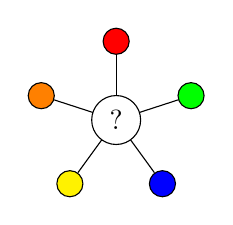
\begin{tikzpicture}
            \foreach[count=\x] \c in {orange,yellow,blue,green,red}
            {
                \node[circle, draw=black, fill=\c] (v\x) at (90+72*\x:1) {};
                \draw (v\x) -- (0,0);
            }
            \node[circle, draw=black, fill=white] at (0,0) {?};
        \end{tikzpicture}
    \end{center}
    
    Es ist direkt erkennbar, dass bei dieser Konstellation die äußeren Knoten niemals unterschiedliche Farben besitzen dürfen, da sonst für den mittleren Knoten eine sechste Farbe benötigt wird. Daher müssen mindestens zwei Knotenpunkte die gleiche Farbe besitzen. Um zu beweisen, dass alles mit fünf Farben einfärbbar ist, wird von von zwei verschiedenen Fällen ausgegangen. Als Beispiel werden hier der orangefarbene und blaue Knoten als Referenz genommen, aber das dient nur zum Zweck der Veranschaulichung. Es kann jeder andere Knoten ebenfalls als Referenz genutzt werden.
    
    \begin{enumerate}
        \item Der orangefarbene Knoten und der blaue Knoten sind \textbf{nicht} durch eine Verbindung verknüpft, die abwechselnd Orange und Gelb ist. Wenn das der Fall ist, dann kann man den blauen Knoten mit einem orangefarbenen ersetzen. Damit ist unsere Bedingung erfüllt und es wurde alles mit fünf Farben eingefärbt.
        
        \begin{center}
            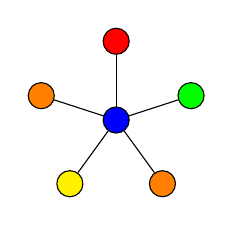
\begin{tikzpicture}
                \foreach[count=\x] \c in {orange,yellow,orange,green,red}
                {
                    \node[circle, draw=black, fill=\c] (v\x) at (90+72*\x:1) {};
                    \draw (v\x) -- (0,0);
                }
                \node[circle, draw=black, fill=blue] at (0,0) {};
            \end{tikzpicture}
        \end{center}
            
        \item Der orangefarbene Knoten und der blaue Knoten sind durch eine Verbindung verknüpft, die abwechselnd orange und blau ist.
        
        \begin{center}
            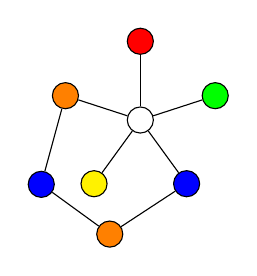
\begin{tikzpicture}
                \node[circle, draw=black, fill=white] (center) at (0,0) {};
                \foreach[count=\x] \c in {orange,yellow,blue,green,red}
                {
                    \node[circle, draw=black, fill=\c] (v\x) at (90+72*\x:1) {};
                    \draw (v\x) -- (center);
                }
                \node[circle, draw=black, fill=blue] (v6) at (90+72+36+15:1.5) {};
                \node[circle, draw=black, fill=orange] (v7) at (90+72+72+36-15:1.5) {};
                \draw[] (v1) -- (v6) -- (v7) -- (v3);
                
            \end{tikzpicture}
        \end{center}
        
        Das heißt, man kann den einen nicht einfach mit dem anderen ersetzen, da sonst ein Konflikt entstehen würde.
        
        \begin{center}
            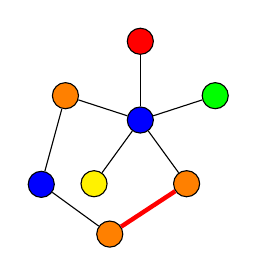
\begin{tikzpicture}
                \node[circle, draw=black, fill=blue] (center) at (0,0) {};
                \foreach[count=\x] \c in {orange,yellow,orange,green,red}
                {
                    \node[circle, draw=black, fill=\c] (v\x) at (90+72*\x:1) {};
                    \draw (v\x) -- (center);
                }
                \node[circle, draw=black, fill=blue] (v6) at (90+72+36+15:1.5) {};
                \node[circle, draw=black, fill=orange] (v7) at (90+72+72+36-15:1.5) {};
                \draw[] (v1) -- (v6) -- (v7);
                \draw[red, ultra thick] (v7) -- (v3);
                
            \end{tikzpicture}
        \end{center}
        
        Man beachte, dass sich der gelbe Knoten innerhalb der Fläche, welche durch die orange/blaue Verbindungskette gebildet wird, befindet. Es gibt keinen Weg um eine Verbindung zum gelben Knoten zu zeichnen, ohne die Verbindungskette zu durchqueren. Dies würde mit der planaren Natur des Graphen im Konflikt stehen.
        
        \begin{center}
            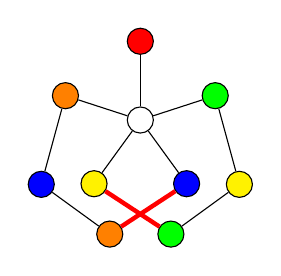
\begin{tikzpicture}
                \node[circle, draw=black, fill=white] (center) at (0,0) {};
                \foreach[count=\x] \c in {orange,yellow,blue,green,red}
                {
                    \node[circle, draw=black, fill=\c] (v\x) at (90+72*\x:1) {};
                    \draw (v\x) -- (center);
                }
                \node[circle, draw=black, fill=blue] (v6) at (90+72+36+15:1.5) {};
                \node[circle, draw=black, fill=orange] (v7) at (90+72+72+36-15:1.5) {};
                
                \node[circle, draw=black, fill=green] (v8) at (90+72+72+36+15:1.5) {};
                \node[circle, draw=black, fill=yellow] (v9) at (90+72+72+72+36-15:1.5) {};
                
                \draw[] (v1) -- (v6) (v6) -- (v7) (v9) -- (v4) (v8) -- (v9);
                \draw[red, ultra thick] (v7) -- (v3) (v2) -- (v8) ;
                
            \end{tikzpicture}
        \end{center}
        
        Daher kann man Fall 1 anwenden, den grünen Knoten mit dem gelben ersetzen und die Mitte entsprechend einfärben.
        
        \begin{center}
            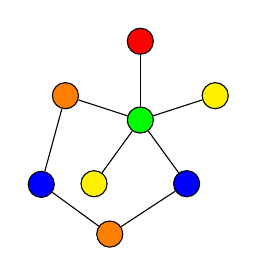
\begin{tikzpicture}
                \node[circle, draw=black, fill=green] (center) at (0,0) {};
                \foreach[count=\x] \c in {orange,yellow,blue,yellow,red}
                {
                    \node[circle, draw=black, fill=\c] (v\x) at (90+72*\x:1) {};
                    \draw (v\x) -- (center);
                }
                \node[circle, draw=black, fill=blue] (v6) at (90+72+36+15:1.5) {};
                \node[circle, draw=black, fill=orange] (v7) at (90+72+72+36-15:1.5) {};
                \draw[] (v1) -- (v6) -- (v7) -- (v3);
                
            \end{tikzpicture}
        \end{center}
    \end{enumerate}
    
    Da in beiden Fällen alles mit fünf Farben eingefärbt werden kann, wirkt sich das rekursiv durch Induktion auf das Hinzufügen der Knoten an den Graphen aus. Somit kann jeder planare Graph mit fünf Farben oder weniger eingefärbt werden.
\end{proof}